\documentclass[a1paper, portrait, fontscale=0.36]{tikzposter}

\usepackage[utf8]{inputenc}
\usepackage[T1]{fontenc}
\usepackage{lmodern}
\usepackage{graphicx}
\usepackage{amsmath, amssymb}
\usepackage{booktabs}
\usepackage{enumitem}
\usepackage{xcolor}
\usepackage{tikz}
\usetikzlibrary{shapes.geometric, arrows.meta, positioning, calc}

% ── Color theme ──────────────────────────────────────────────
\definecolor{DarkNavy}{HTML}{0D1B2A}
\definecolor{MidNavy}{HTML}{1B2838}
\definecolor{AccentBlue}{HTML}{1976D2}
\definecolor{AccentGold}{HTML}{F9A825}
\definecolor{LightGray}{HTML}{E8EDF2}
\definecolor{CardGreen}{HTML}{1B5E20}
\definecolor{FeltGreen}{HTML}{2E7D32}
\definecolor{ChipRed}{HTML}{C62828}
\definecolor{ChipBlue}{HTML}{1565C0}

% ── tikzposter theme ─────────────────────────────────────────
\usetheme{Default}

\definecolorstyle{PokerStyle}{
  \definecolor{colorOne}{named}{DarkNavy}
  \definecolor{colorTwo}{named}{AccentBlue}
  \definecolor{colorThree}{named}{AccentGold}
}{
  \colorlet{backgroundcolor}{white}
  \colorlet{framecolor}{AccentBlue}
  \colorlet{titlefgcolor}{white}
  \colorlet{titlebgcolor}{DarkNavy}
  \colorlet{blocktitlebgcolor}{AccentBlue}
  \colorlet{blocktitlefgcolor}{white}
  \colorlet{blockbodybgcolor}{white}
  \colorlet{blockbodyfgcolor}{DarkNavy}
  \colorlet{innerblocktitlebgcolor}{LightGray}
  \colorlet{innerblocktitlefgcolor}{DarkNavy}
  \colorlet{innerblockbodybgcolor}{white}
  \colorlet{innerblockbodyfgcolor}{DarkNavy}
  \colorlet{notebgcolor}{AccentGold}
  \colorlet{notefgcolor}{DarkNavy}
  \colorlet{notefrcolor}{AccentGold}
}
\usecolorstyle{PokerStyle}

\useblockstyle{Default}

% ── Title ────────────────────────────────────────────────────
\title{\textbf{Multi-Agent Reinforcement Learning\\for No-Limit Texas Hold'em}}
\author{Al\'{e}o Ibrahim Houmed \quad \& \quad Maxence Adly}
\institute{Reinforcement Learning Group Project}

\begin{document}

\maketitle

% ══════════════════════════════════════════════════════════════
%  ROW 1: Introduction | Game & Environment
% ══════════════════════════════════════════════════════════════

\begin{columns}

\column{0.5}

\block{1. Introduction \& Motivation}{
  \textbf{No-Limit Texas Hold'em (NLHE)} is one of the most challenging domains in AI due to its combination of:
  \begin{itemize}[leftmargin=1.5em, itemsep=4pt]
    \item \textbf{Imperfect information} -- players cannot see opponents' cards
    \item \textbf{Stochastic dynamics} -- card dealing introduces randomness
    \item \textbf{Large action space} -- bet sizing creates combinatorial complexity
    \item \textbf{Multi-agent competition} -- opponents adapt their strategies
    \item \textbf{Sparse, delayed rewards} -- outcomes only at hand conclusion
  \end{itemize}

  \vspace{0.5em}
  We train autonomous agents to play NLHE through \textbf{self-play reinforcement learning}, where a single shared policy improves by competing against copies of itself. This approach has proven effective in games like Go (AlphaGo/Zero) and poker (Pluribus, DeepStack).

  \vspace{0.5em}
  \textbf{Key contributions:}
  \begin{itemize}[leftmargin=1.5em, itemsep=3pt]
    \item Custom multi-agent NLHE environment supporting 2--10 players
    \item PPO training with action masking for legal move enforcement
    \item Cash-game mode with persistent stacks and player elimination
    \item Interactive GUI and CLI tools for model evaluation
  \end{itemize}
}

\column{0.5}

\block{2. Game \& Environment Design}{
  \begin{tikzpicture}[
    box/.style={draw, rounded corners=4pt, minimum width=3.8cm, minimum height=1.2cm, 
                text centered, font=\small\bfseries, line width=1pt},
    arrow/.style={-{Stealth[length=3mm]}, line width=1.2pt, AccentBlue}
  ]
    \node[box, fill=LightGray, draw=DarkNavy] (deal) at (0,0) {Deal Cards};
    \node[box, fill=LightGray, draw=DarkNavy] (pre) at (5.5,0) {Preflop};
    \node[box, fill=LightGray, draw=DarkNavy] (flop) at (11,0) {Flop};
    \node[box, fill=LightGray, draw=DarkNavy] (turn) at (16.5,0) {Turn};
    \node[box, fill=LightGray, draw=DarkNavy] (river) at (22,0) {River};
    \node[box, fill=AccentGold!30, draw=AccentGold!80!black] (show) at (27.5,0) {Showdown};
    
    \draw[arrow] (deal) -- (pre);
    \draw[arrow] (pre) -- (flop);
    \draw[arrow] (flop) -- (turn);
    \draw[arrow] (turn) -- (river);
    \draw[arrow] (river) -- (show);
  \end{tikzpicture}

  \vspace{0.5em}
  \textbf{Environment specifications:}

  \vspace{0.3em}
  \begin{minipage}[t]{0.48\linewidth}
    \textbf{Observation Space} (per player):
    \begin{itemize}[leftmargin=1.2em, itemsep=2pt, font=\small]
      \item Hole cards (one-hot, 52-dim)
      \item Board cards (multi-hot, 52-dim)
      \item Street indicator (one-hot, 4-dim)
      \item Position relative to dealer
      \item Normalised stacks, pot, bets
      \item Min/max raise amounts
      \item Per-street betting history
    \end{itemize}
    All values normalised to $[0, 1]$.
  \end{minipage}%
  \hfill
  \begin{minipage}[t]{0.48\linewidth}
    \textbf{Action Space} (6 discrete actions):

    \vspace{0.3em}
    \renewcommand{\arraystretch}{1.3}
    \begin{tabular}{@{}cl@{}}
      \toprule
      \textbf{Idx} & \textbf{Action} \\
      \midrule
      0 & Fold \\
      1 & Check / Call \\
      2 & Raise Minimum \\
      3 & Raise $\frac{1}{2}$ Pot \\
      4 & Raise Pot \\
      5 & All-In \\
      \bottomrule
    \end{tabular}

    \vspace{0.5em}
    \textbf{Reward:} $r_i = \text{stack}_i^{\text{final}} - \text{stack}_i^{\text{initial}}$ \\
    Sparse, zero-sum at hand end.
  \end{minipage}
}

\end{columns}

% ══════════════════════════════════════════════════════════════
%  ROW 2: Method | Model Architecture
% ══════════════════════════════════════════════════════════════

\begin{columns}

\column{0.5}

\block{3. Method: PPO with Self-Play}{
  We use \textbf{Proximal Policy Optimization (PPO)} within the \textbf{Ray RLlib} framework, employing a single shared policy for all agents (\textit{self-play}).

  \vspace{0.5em}
  \textbf{PPO Objective} (clipped surrogate):
  \[
    L^{\text{CLIP}}(\theta) = \hat{\mathbb{E}}_t \left[ \min\!\left( r_t(\theta)\, \hat{A}_t,\; \text{clip}(r_t(\theta), 1{-}\epsilon, 1{+}\epsilon)\, \hat{A}_t \right) \right]
  \]
  where $r_t(\theta) = \frac{\pi_\theta(a_t|s_t)}{\pi_{\theta_{\text{old}}}(a_t|s_t)}$ and $\hat{A}_t$ is the GAE advantage estimate.

  \vspace{0.5em}
  \textbf{Action Masking:} Illegal actions are suppressed by setting their logits to $-10^{38}$ before the softmax, guaranteeing $\pi(a|s) = 0$ for illegal moves:
  \[
    \ell_i' = \begin{cases} \ell_i & \text{if action } i \text{ is legal} \\ -10^{38} & \text{otherwise} \end{cases}
  \]

  \vspace{0.5em}
  \renewcommand{\arraystretch}{1.25}
  \begin{tabular}{@{}ll@{}}
    \toprule
    \textbf{Hyperparameter} & \textbf{Value} \\
    \midrule
    Learning rate & $3 \times 10^{-4}$ \\
    Discount $\gamma$ & $1.0$ (episodic) \\
    GAE $\lambda$ & $0.95$ \\
    Clip parameter $\epsilon$ & $0.2$ \\
    Entropy coefficient & $0.02$ \\
    VF loss coefficient & $0.5$ \\
    Train batch size & $4096$ \\
    Minibatch size & $256$ \\
    SGD epochs per update & $4$ \\
    Rollout workers & $2$ \\
    \bottomrule
  \end{tabular}
}

\column{0.5}

\block{4. Neural Network Architecture}{
  \vspace{0.3em}
  \begin{center}
  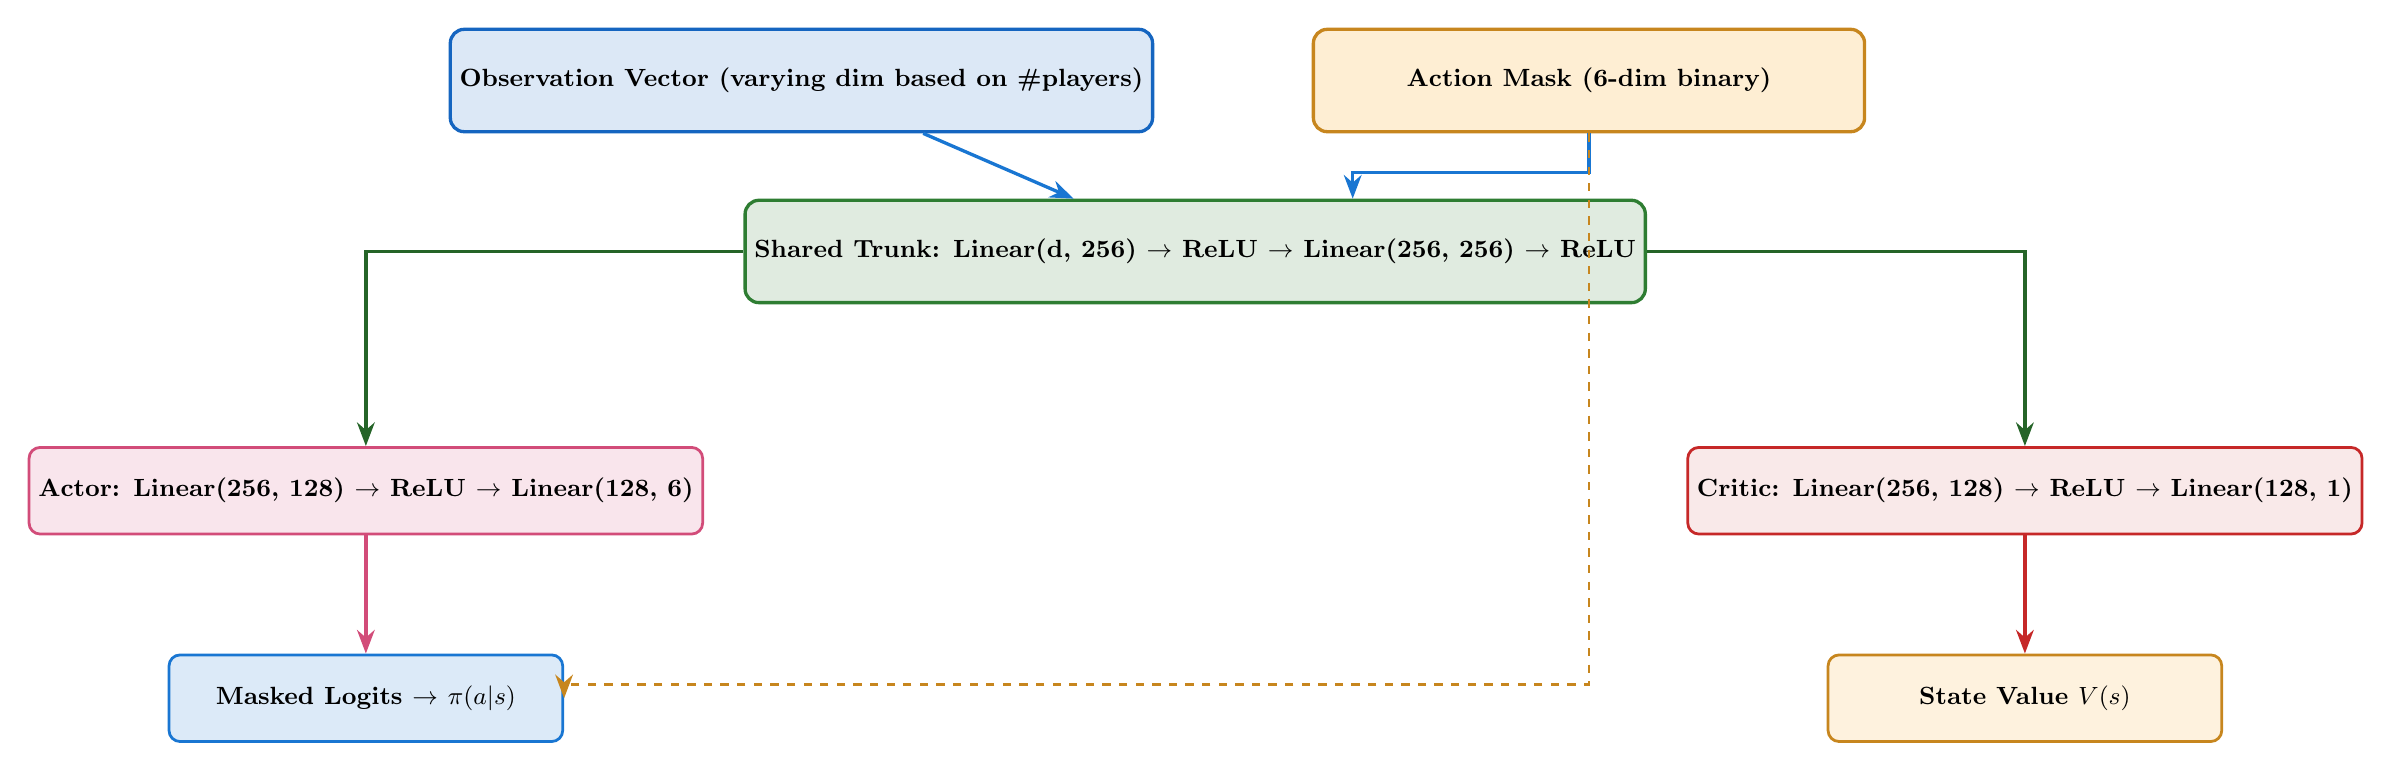
\begin{tikzpicture}[
    node distance=1.4cm,
    box/.style={draw, rounded corners=5pt, minimum width=7cm, minimum height=1.3cm, 
                text centered, font=\small\bfseries, line width=1.2pt},
    smallbox/.style={draw, rounded corners=4pt, minimum width=5cm, minimum height=1.1cm, 
                     text centered, font=\small\bfseries, line width=1pt},
    arrow/.style={-{Stealth[length=3mm]}, line width=1.2pt},
    dasharrow/.style={-{Stealth[length=3mm]}, line width=1pt, dashed}
  ]
    % Input layer
    \node[box, fill=ChipBlue!15, draw=ChipBlue] (obs) {Observation Vector (varying dim based on \#players)};
    \node[box, fill=AccentGold!20, draw=AccentGold!80!black, right=2cm of obs] (mask) {Action Mask (6-dim binary)};
    
    % Trunk
    \node[box, fill=FeltGreen!15, draw=FeltGreen, below=1.5cm of $(obs)!0.5!(mask)$] (trunk) 
      {Shared Trunk: Linear(d, 256) $\to$ ReLU $\to$ Linear(256, 256) $\to$ ReLU};
    
    % Heads
    \node[smallbox, fill=purple!10, draw=purple!70, below left=1.8cm and 0.5cm of trunk] (actor) 
      {Actor: Linear(256, 128) $\to$ ReLU $\to$ Linear(128, 6)};
    \node[smallbox, fill=ChipRed!10, draw=ChipRed, below right=1.8cm and 0.5cm of trunk] (critic) 
      {Critic: Linear(256, 128) $\to$ ReLU $\to$ Linear(128, 1)};
    
    % Outputs
    \node[smallbox, fill=AccentBlue!15, draw=AccentBlue, below=1.5cm of actor] (logits)
      {Masked Logits $\to$ $\pi(a|s)$};
    \node[smallbox, fill=AccentGold!15, draw=AccentGold!80!black, below=1.5cm of critic] (value)
      {State Value $V(s)$};
    
    % Arrows
    \draw[arrow, AccentBlue] (obs) -- (trunk);
    \draw[arrow, AccentBlue] (mask.south) -- ++(0,-0.5) -| ($(trunk.north)+(2,0)$);
    \draw[arrow, FeltGreen!80!black] (trunk) -| (actor);
    \draw[arrow, FeltGreen!80!black] (trunk) -| (critic);
    \draw[arrow, purple!70] (actor) -- (logits);
    \draw[arrow, ChipRed] (critic) -- (value);
    \draw[dasharrow, AccentGold!80!black] (mask.south) -- ++(0,-0.5) -| ++(0, -6.5) -| (logits.east)
      node[midway, right, font=\footnotesize\itshape, text=AccentGold!80!black] {};

  \end{tikzpicture}
  \end{center}

  \vspace{0.3em}
  The \textbf{PokerActionMaskRLModule} extends RLlib's \texttt{DefaultPPOTorchRLModule}:
  \begin{itemize}[leftmargin=1.5em, itemsep=3pt]
    \item \textbf{Shared trunk}: Extracts features from the observation vector
    \item \textbf{Actor head}: Produces 6-dimensional logits, masked for legality
    \item \textbf{Critic head}: Outputs scalar baseline value $V(s)$ for variance reduction
    \item Total parameters: $\sim$200K (lightweight, fast inference)
  \end{itemize}
}

\end{columns}

% ══════════════════════════════════════════════════════════════
%  ROW 3: Training Results
% ══════════════════════════════════════════════════════════════

\block{5. Training Results (60 Iterations, 245K Timesteps, 2-Player Self-Play)}{
  \begin{center}
    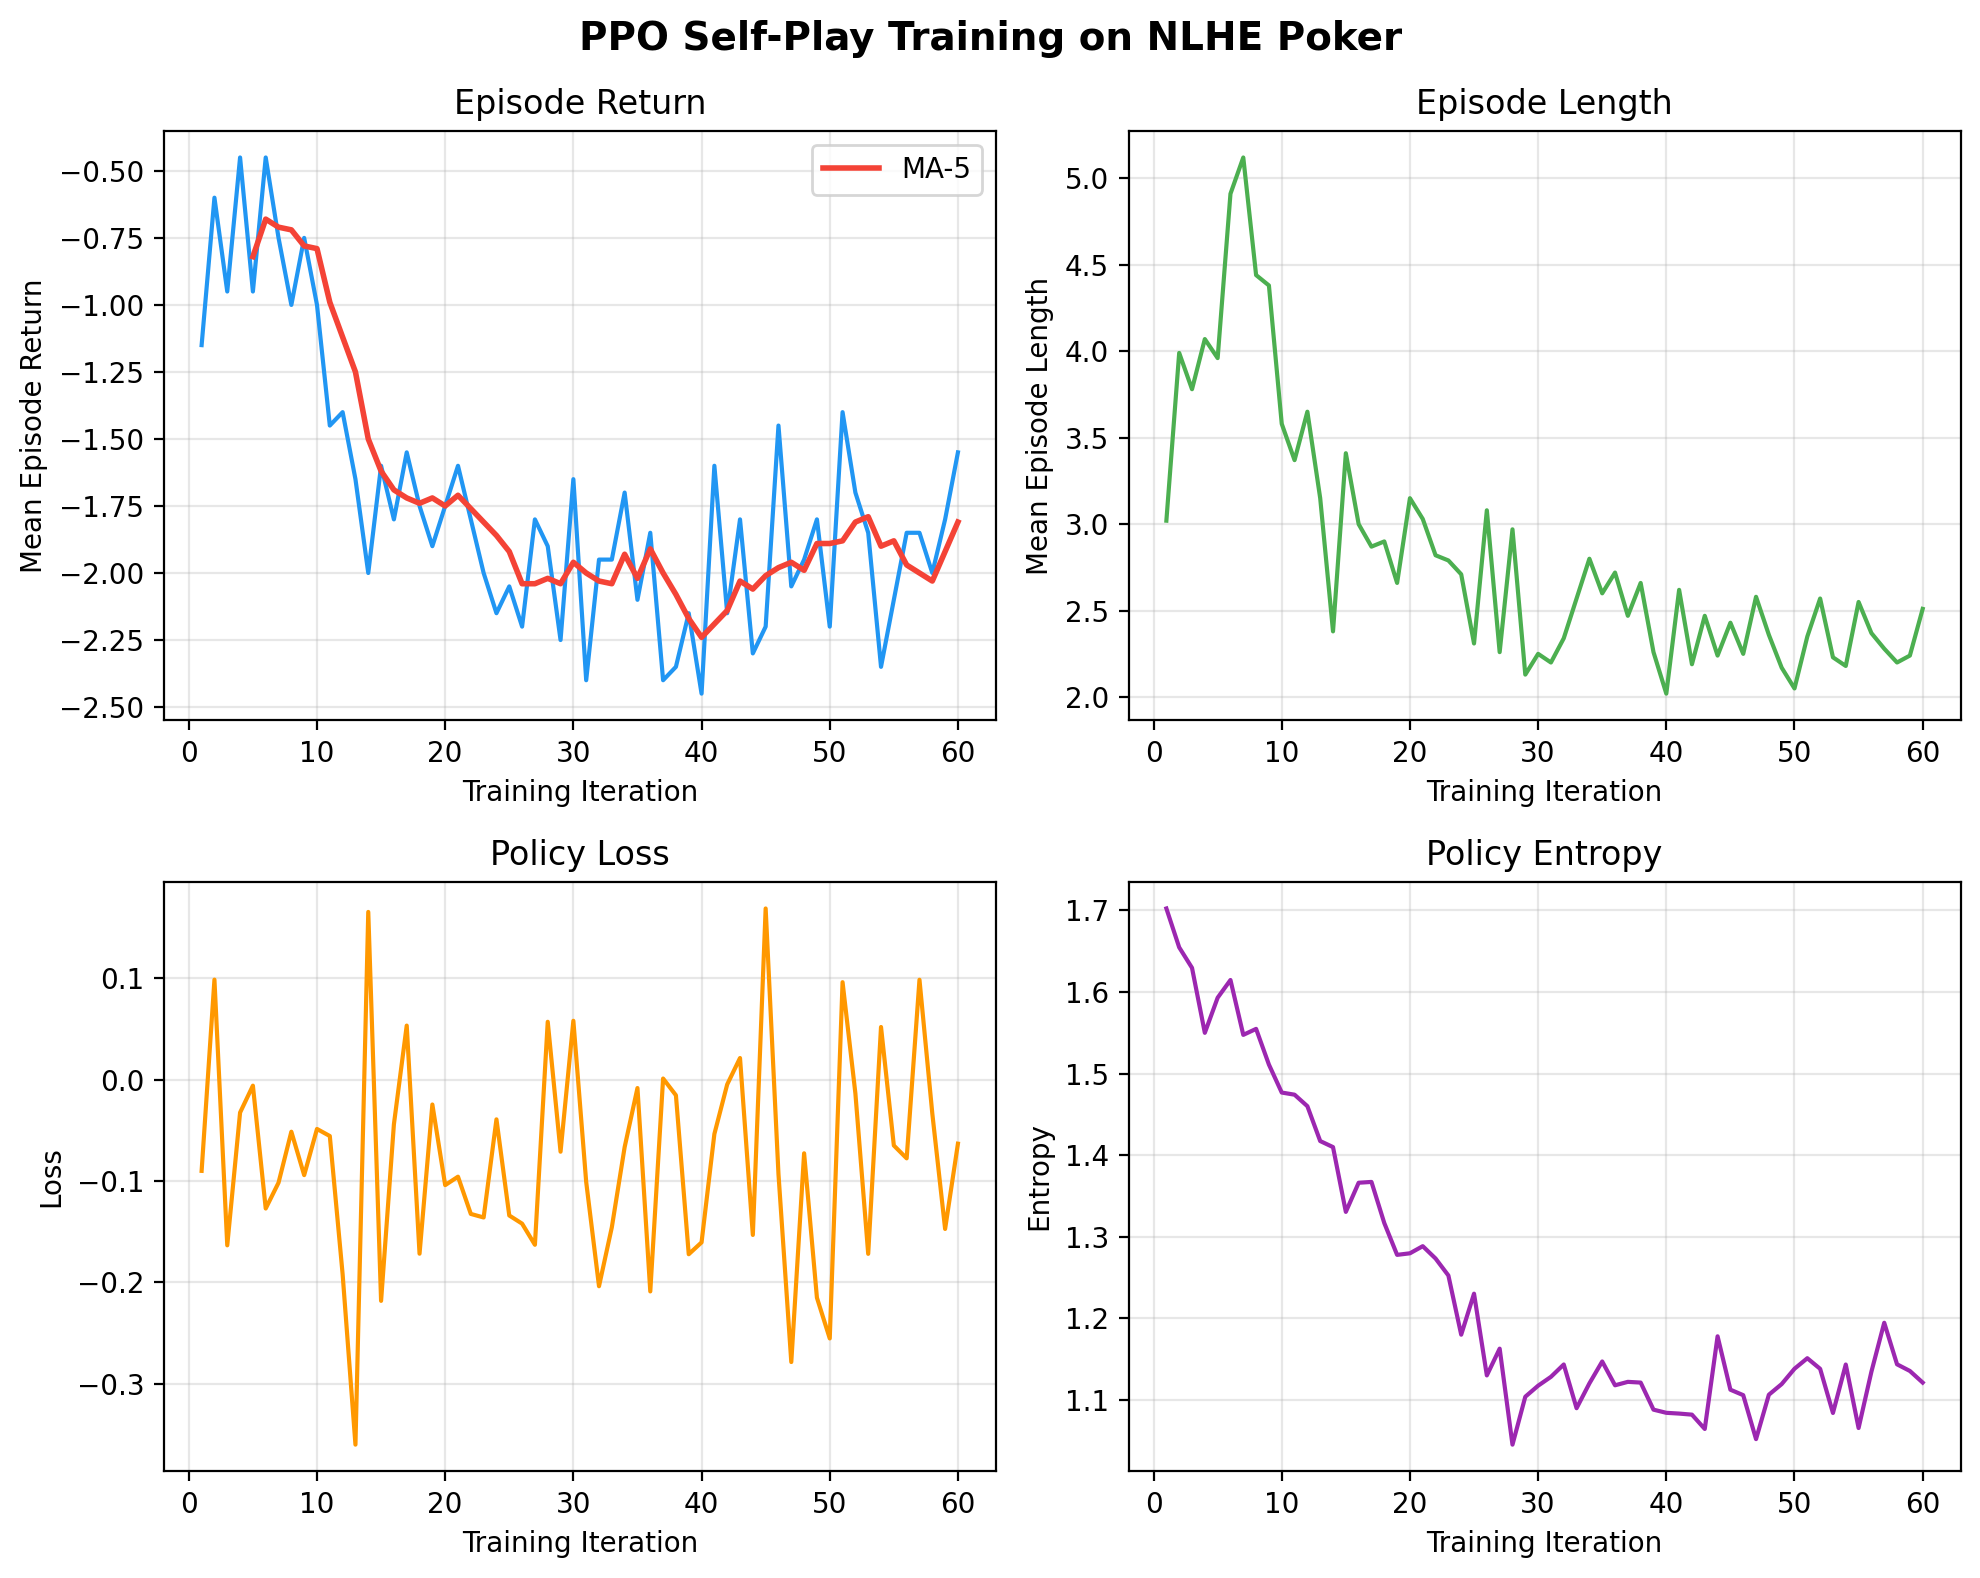
\includegraphics[width=0.85\linewidth]{training_curves.png}
  \end{center}

  \vspace{0.3em}
  \begin{minipage}[t]{0.48\linewidth}
    \textbf{Observations:}
    \begin{itemize}[leftmargin=1.5em, itemsep=3pt]
      \item Episode return oscillates around zero as expected in \textbf{zero-sum self-play} -- the policy plays against itself, so gains and losses cancel
      \item Episode length stabilises around 2--3 steps, consistent with heads-up NLHE where many hands end quickly (pre-flop fold or all-in)
    \end{itemize}
  \end{minipage}
  \hfill
  \begin{minipage}[t]{0.48\linewidth}
    \textbf{Training dynamics:}
    \begin{itemize}[leftmargin=1.5em, itemsep=3pt]
      \item \textbf{Policy loss} converges with stable gradient updates
      \item \textbf{Entropy} decreases from $\sim$1.6 to $\sim$1.1, indicating the policy becomes more decisive while retaining exploration
      \item Training completed over \textbf{245,760 environment steps} across 60 PPO iterations
    \end{itemize}
  \end{minipage}
}

% ══════════════════════════════════════════════════════════════
%  ROW 4: Evaluation | Action Distribution
% ══════════════════════════════════════════════════════════════

\begin{columns}

\column{0.5}

\block{6. Evaluation: PPO Agent vs Random Opponent}{
  \begin{center}
    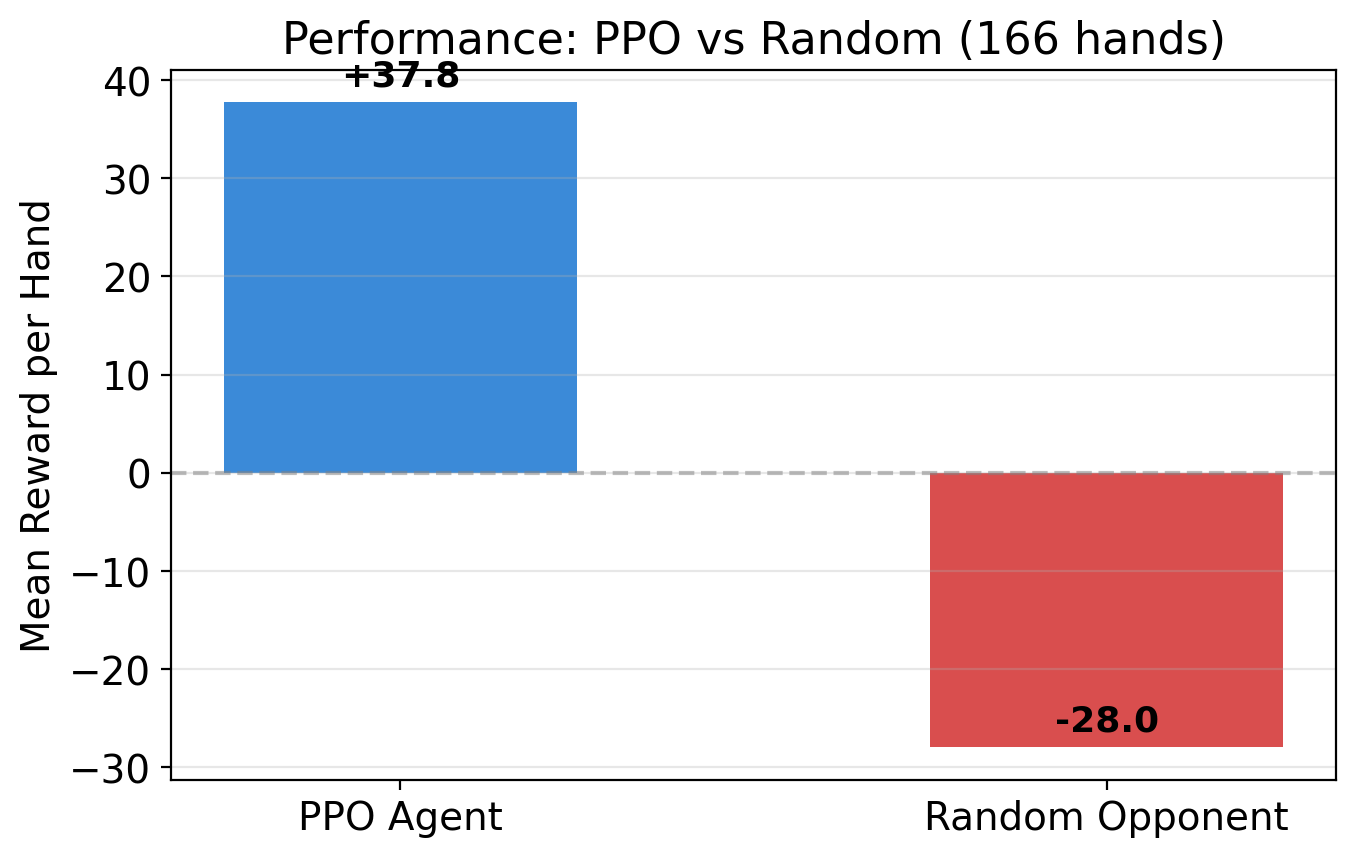
\includegraphics[width=0.75\linewidth]{plot_eval_bars.png}
  \end{center}

  \vspace{0.3em}
  \renewcommand{\arraystretch}{1.3}
  \begin{tabular}{@{}lcc@{}}
    \toprule
    \textbf{Metric} & \textbf{PPO Agent} & \textbf{Random} \\
    \midrule
    Mean reward/hand & $\mathbf{+37.8}$ & $-28.0$ \\
    Total reward (166 hands) & $+6{,}270$ & $-4{,}640$ \\
    Win rate (reward $> 0$) & $21.1\%$ & -- \\
    \bottomrule
  \end{tabular}

  \vspace{0.5em}
  The trained PPO agent significantly outperforms a uniformly random baseline, earning an average of \textbf{+37.8 chips/hand}. Despite a modest win rate (21.1\%), the agent wins \emph{larger pots} when it does win, showing it has learned to extract value from strong hands.
}

\column{0.5}

\block{7. Learned Action Distribution}{
  \begin{center}
    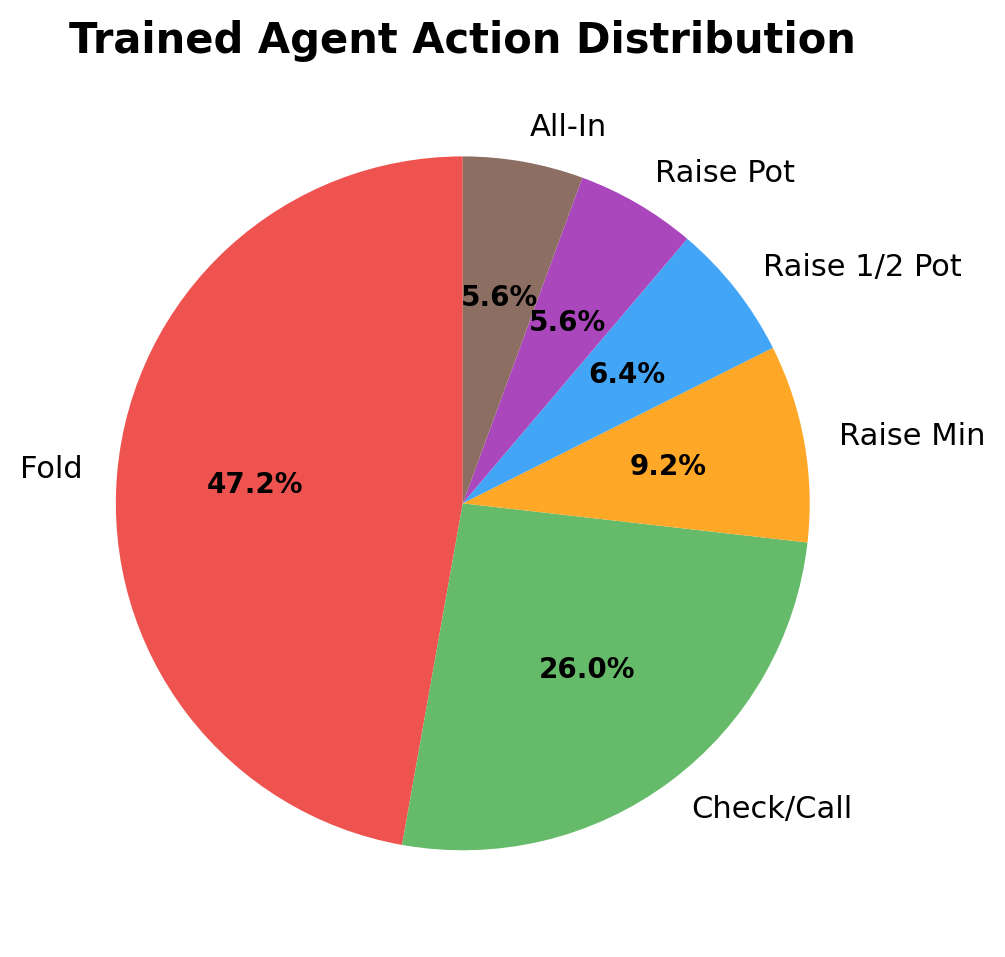
\includegraphics[width=0.6\linewidth]{plot_action_dist.png}
  \end{center}

  \vspace{0.3em}
  The trained policy exhibits \textbf{tight-aggressive} characteristics:
  \begin{itemize}[leftmargin=1.5em, itemsep=3pt]
    \item \textbf{Fold (47.2\%)} -- High fold rate shows selectivity; the agent does not chase weak hands
    \item \textbf{Check/Call (26.0\%)} -- Pot control with marginal holdings
    \item \textbf{Raise actions (20.8\%)} -- Combined raising frequency shows willingness to build pots with strong hands
    \item \textbf{All-In (5.6\%)} -- Reserved for premium situations
  \end{itemize}

  \vspace{0.3em}
  This distribution resembles strategies recommended in poker theory: fold weak hands early, play strong hands aggressively.
}

\end{columns}

% ══════════════════════════════════════════════════════════════
%  ROW 5: Technical Stack | Conclusions
% ══════════════════════════════════════════════════════════════

\begin{columns}

\column{0.5}

\block{8. Technical Stack \& Implementation}{
  \renewcommand{\arraystretch}{1.3}
  \begin{tabular}{@{}p{6cm}p{14cm}@{}}
    \toprule
    \textbf{Component} & \textbf{Technology} \\
    \midrule
    RL Framework & Ray RLlib 2.54 (new API stack: RLModule + Learner + ConnectorsV2) \\
    Algorithm & PPO with GAE ($\lambda = 0.95$, $\gamma = 1.0$) \\
    Deep Learning & PyTorch 2.10 \\
    Environment & Custom Gymnasium-based \texttt{MultiAgentEnv} \\
    Hand Evaluation & Treys library (7,462 hand equivalence classes) \\
    Training Mode & Self-play with single shared policy \\
    Game Modes & Single-hand (tournament) and cash-game (persistent stacks) \\
    Interfaces & CLI training/evaluation + Tkinter GUI viewer \\
    \bottomrule
  \end{tabular}

  \vspace{0.5em}
  \textbf{Multi-agent design:} All $N$ players share one policy (\texttt{shared\_policy}). The environment is turn-based: each \texttt{step()} involves exactly one agent acting. This ensures the policy generalises across all table positions.
}

\column{0.5}

\block{9. Conclusions \& Future Work}{
  \textbf{Summary of Results:}
  \begin{itemize}[leftmargin=1.5em, itemsep=4pt]
    \item Successfully trained a PPO agent to play legal, strategic NLHE poker through self-play
    \item Action masking guarantees 100\% legal play at all times
    \item The agent learns a \textbf{tight-aggressive} strategy, significantly outperforming random opponents ($+37.8$ chips/hand average)
    \item The policy develops meaningful action preferences (selective folding, value betting)
    \item Cash-game mode enables training with realistic stack dynamics and elimination
  \end{itemize}

  \vspace{0.5em}
  \textbf{Future Directions:}
  \begin{itemize}[leftmargin=1.5em, itemsep=4pt]
    \item Scale to 6--10 player tables and longer training horizons
    \item Implement \textbf{population-based training} to avoid strategy collapse
    \item Add \textbf{opponent modelling} (separate policy per archetype)
    \item Integrate \textbf{Counterfactual Regret Minimisation (CFR)} as a baseline comparison
    \item Incorporate continuous bet sizing for finer-grained strategy
    \item Evaluate against established poker AI benchmarks (Slumbot, etc.)
  \end{itemize}
}

\end{columns}

\end{document}
